% --------------------
  \chapter{Diseño}
% --------------------
\label{C:desarrollo}

En la presente sección se diseñará la aplicación y los componentes necesarios para que funcione de forma adecuada. Es necesario establecer que para poder diseñar la aplicación fue necesario realizar una distribución de las funciones de la misma por medio de distintos componentes. Asegurando así que se tenga pruebas de que cada componente tiene un funcionamiento correcto por separado como en conjunto. En la figura (\ref{appdiagram}), se puede ver como se distribuyó el diseño de la aplicación.
\begin{figure}[H]
    \centering
    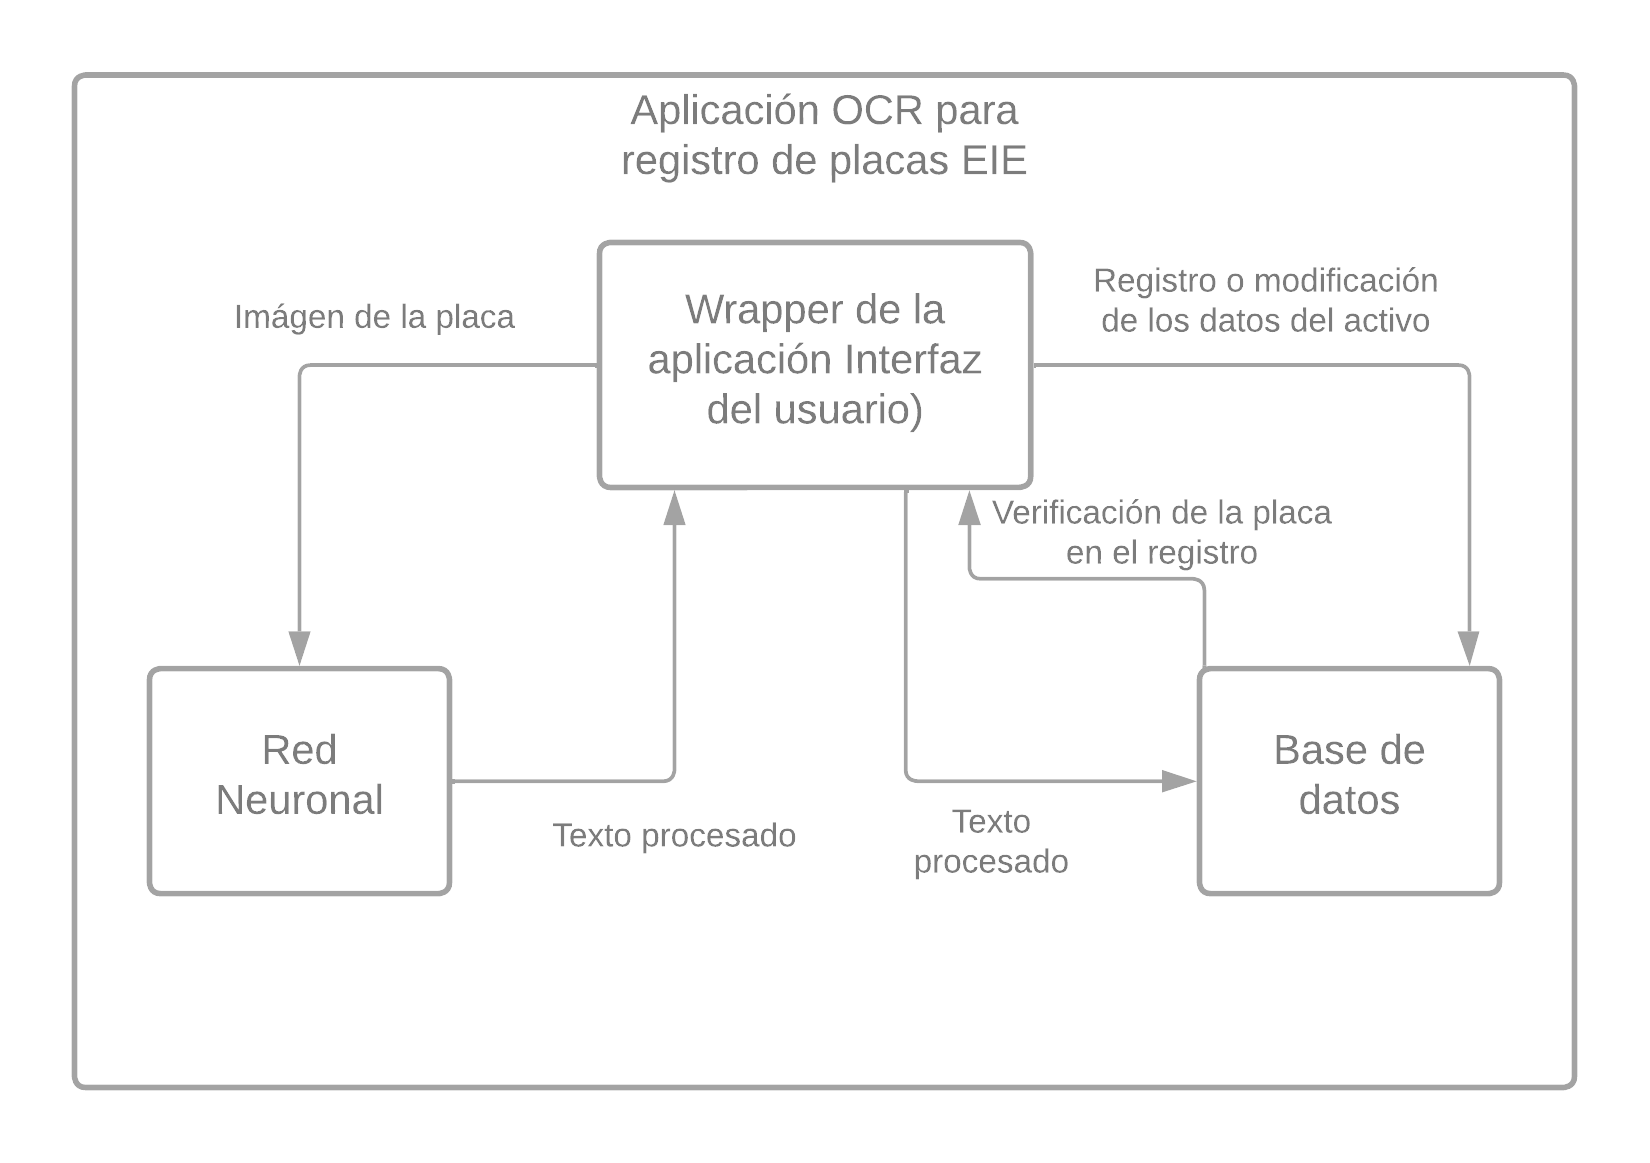
\includegraphics[width=0.7\textwidth]{imagenes/diseño/diagrama_del_programa.png}
    \caption{Diagrama del funcionamiento de la aplicación (creación propia)}
    \label{appdiagram}
\end{figure}
\par
Se crearon tres principales componentes para la aplicación, donde la principal sería el wrapper o la interfaz del usuario, la red neuronal y la base de datos. Los tres componentes están conectados entre sí por medio del wrapper, que no solamente permite las entradas y las salidas con los usuarios, sino que también corre las funciones para acceder a cada uno de los componentes.

\section{Red neuronal}
Debido a la complejidad y cantidad de recursos que puede requerir crear una red neuronal completamente de cero, se optó por utilizar una red neuronal pre-fabricada, a la cual se le modificasen diferentes parámetros para procesar específicamente imágenes y que realizaran un análisis de OCR. 
\par
El servicio utilizado para este proyecto fue el de Nanonets, debido a que las redes neuronales que ofrecen permiten nativamente adaptarlas para el reconocimiento y procesamiento de caracteres. Específicamente se consideró el pre-procesamiento de las imágenes y el procesado como los más significativos a la hora de alterar las especificaciones buscadas dentro de lo que iba a analizar la red.
\par
Primeramente se escogió que el modelo de red más adecuado era el de OCR. Luego se permite moficar el tipo de preprocesado que reciben las imágenes una vez que son recibidas por el servidor.
\par
El primer parámetro a corregir es la normalización de la imagen, la cual sirve para cambiar la intensidad de los pixeles a uno adecuado. Luego la corrección de torcimiento (Skew correction), que en caso de que la imagen recibida esté torcida permita verla con un mejor ángulo. La reducción de ruido, que intenta minizar el ruido en la imagen. Por último se tomó en cuenta la aplicación de escala de grises y binarización de la imágen para que resalte de forma correcta el texto de las placas.
\par
Es necesario destacar que no fue necesaria la implementación de código para realizar ninguna de las funciones de pre-procesado ni tampoco para los parámetros del procesado de la red. Lo siguiente llevado a cabo fue la definición del tipo de elementos que debería buscar específicamente la red para devolver como respuesta a la salida. Para ello se pusieron parámetros que eliminasen todo tipo de texto y elementos que no correspondieran a un número y que solamente analizara una única línea, debido a que al ser OCR, podría buscar devolver un texto más grande del necesario. Todo esto es necesario debido a que las placas de la Universidad de Costa Rica (figura \ref{ejem_placa}), poseen no solamente el número de activo, sino que también el logo y nombre de la Universidad.
\begin{figure}[H]
    \centering
    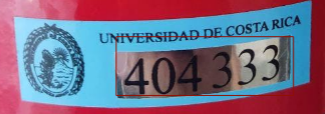
\includegraphics[width=0.5\textwidth]{imagenes/diseño/ejem_placa.PNG}
    \caption{Placa de activo de la Universidad de Costa Rica (ejemplo)}
    \label{ejem_placa}
\end{figure}
\par
La última parte del diseño de la red es el entrenamiento de la misma, por medio de alimentación de datos de entrada. En este caso se utilizó un total de 30 placas capturadas en diferentes activos a través de la facultad de ingeniería y de la EIE. El modelo visto en la Figura \ref{ejem_placa} no es el único existente, sino que se encuentran modelos más antiguos, éstos también fueron considerados dentro del entrenamiento para tener una amplia gama de respuesta por parte de la red. 
\par
Una vez terminado el proceso de entrenamiento se diseñó un código capaz de interactuar con la API de Nanonets, que recibe las imágenes, en este caso en forma de archivo binario, para poder procesarla por medio de la red. La API devuelve una salida con diferentes parámetros escaneados de la imagen en formato JSON, pero únicamente se tomó en cuenta el \lstinline{ocr_text}. La conexión se realizó por medio de el paquete de requests, que permite realizar solicitudes a servidores y servicios API utilizando una llave personal para acceder a ellas (la llave fue provista por Nanonets para la implementación de la aplicación). A continuación se muestran el código de conexión al servidor y para extraer la respuesta respectivamente: 

\begin{lstlisting}[language=Python,frame=single,caption=Código para envío de las placas y recibimiento del texto de la misma (creación propia), inputencoding=latin1]
url = 'https://app.nanonets.com/api/v2/OCR/Model/34353217-1d3f-4511-b86f-e24e842e66e8/LabelFile/?async=false'
data = {'file': open(self.captura_actual, 'rb')}
response = requests.post(url, auth=requests.auth.HTTPBasicAuth('0DeaHQHCf7qAs9n7mFAGmF9gHd6IVMA9', ''), files=data)
\end{lstlisting}

\begin{lstlisting}[language=Python,frame=single,caption=Código para extracción del texto de la placa de la respuesta de la red neuronal (creación propia), inputencoding=latin1]
self.placa_actual = response_json["result"][0]['prediction'][0]['ocr_text']
\end{lstlisting}

\section{Base de datos}
La base de datos se diseñó pensando en que se debía tener un modelo intuitivo que fuese fácil de manipular, donde los datos pudiesen ser exportados de manera sencilla a algún formato conocido por los usuarios. Por ello se utilizó una base de datos relacional, que constará de únicamente una tabla, la cual está definida como la tabla \ref{table1}. 
\begin{table}[H]
\centering
\resizebox{\columnwidth}{!}{\begin{tabular}{cccc}
\hline
Placa (primary key)        & ubicación                    & tipo de activo           & descripción                              \\ \hline
Número de placa del activo & Donde se encuentra el activo & Clasificación del activo & Descripción más detallada de los activos \\ \hline
\end{tabular}}
\caption{Tabla implementada en la base de datos}
\label{table1}
\end{table}

\par
Para la creación de la tabla se instaló un servidor local por medio de la herramienta MySQL, que permitiera realizar la base de datos sin importarla a un servidor remoto online para realizar las pruebas necesarias dentro del desarrollo de la aplicación. La creación de la tabla dentro de la base de datos se realizó por medio de un script de Python que accediera a la base de datos y generara una solicitud para una tabla nueva con las columnas definidas previamente. El script además dentro de la creación de las columnas define el \textit{Primary Key}, que representa la identificación de cada uno de los registros, no es necesario hacer una asignación automática, puesto que se utilizaría la placa como identificación de cada uno de los registros. El paquete de python utilizado para la gestión de bases de datos fue el nativo de MySQL llamado MySQL Connector, este se instaló dentro del paquete de MYSQL community. El código del script de Python implementado se puede ver a continuación:
\newpage
\begin{lstlisting}[language=Python,frame=single,caption= Script de python para la conexión a una base de datos (creación propia), inputencoding=latin1]
import mysql.connector

db = mysql.connector.connect(
    host='localhost',
    user='root',
    passwd='InventarioEIE2409',
    database='inventarioeie'
)
mycursor = db.cursor()
\end{lstlisting}
\par
Esta sección de código realiza una conexión simple al servidor local de la base de datos, con los credenciales del usuario root para pdoer tener manejo completo de la misma. Dentro de los accesos realizados más adelante no es necesario utilizar una acceso root, puesto que no se estará modificando la tabla y su estructura, sino únicamente añadiendo y modificando datos dentro. Además crea un cursor, el cual es el encargado de realizar todas las operaciones para la creación de bases de datos, tablas y toda la inserción, eliminación y modificación de datos en general, es decir maneja cada una de las solicitudes a la BD. 
\begin{lstlisting}[language=Python,frame=single,caption= Script de python para la creación de una tabla en una base de datos (creación propia), inputencoding=latin1]
mycursor.execute("CREATE TABLE Activos (placa int PRIMARY KEY, ubicacion TEXT(65535), tipo_de_activo TEXT(65535), descripcion TEXT(65535))")
\end{lstlisting}
\par
La anterior sección del script, únicamente creó la tabla nueva llamada \textbf{Activos}, con todos los parámetros necesarios, definiendo así donde se almacenarían los datos a futuro. Los valores que se dieron al tipo de variable de cada una de las columnas es la longitud que puede tener la misma. Para asegurar una generalidad y funcionamiento seguro, se utilizó el valor máximo para cada tipo de variable (65535 caracteres).
\par
Todas y cada una de las funciones que gestionan los accesos y las escrituras a la base de datos se implementaron como funciones dentro del wrapper de la aplicación, ya que es necesario que el funcionamiento se de durante el uso de la aplicación. 




\section{Wrapper de la aplicación}